%% ARTIGO 3 - ADAPTACAO TRANSCULTURAL DO WOCAT-SLM (WOCAT-SLM-QBR)
%
% ======================================================================
% PENDENCIAS QUE EXIGEM DADOS OU VERIFICACAO ANTES DA SUBMISSAO
% ======================================================================
% [ ] Concluir a retrotraducao (Etapa 3) e arquivar os relatorios BT1 e BT2.
% [ ] Reportar o IVC por item, o kappa de Fleiss e as decisoes de retencao apos o julgamento do comite de especialistas.
% [ ] Redigir os itens da secao 9 e submete-los ao comite na Etapa 4.
% [ ] Inserir o numero do processo da bolsa CNPq.
% [ ] Confirmar a versao do ATLAS.ti empregada.
% ======================================================================


% Template for Elsevier journal article Ecological Economics
% version 1.2 dated 09 May 2011

% This file (c) 2009-2011 Elsevier Ltd.  Modifications may be freely made,
% provided the edited file is saved under a different name

% This file contains modifications for Ecological Economics
% but may easily be adapted to other journals

% Changes since version 1.1
% - added "procedia" option compliant with ecrc.sty version 1.2a
%   (makes the layout approximately the same as the Word CRC template)
% - added example for generating copyright line in abstract

%-----------------------------------------------------------------------------------

%% This template uses the elsarticle.cls document class and the extension package ecrc.sty
%% For full documentation on usage of elsarticle.cls, consult the documentation "elsdoc.pdf"
%% Further resources available at http://www.elsevier.com/latex

%-----------------------------------------------------------------------------------

%%%%%%%%%%%%%%%%%%%%%%%%%%%%%%%%%%%%%%%%%%%%%%%%%%%%%%%%%%%%%%
%%%%%%%%%%%%%%%%%%%%%%%%%%%%%%%%%%%%%%%%%%%%%%%%%%%%%%%%%%%%%%
%%                                                          %%
%% Important note on usage                                  %%
%% -----------------------                                  %%
%% This file should normally be compiled with PDFLaTeX      %%
%% Using standard LaTeX should work but may produce clashes %%
%%                                                          %%
%%%%%%%%%%%%%%%%%%%%%%%%%%%%%%%%%%%%%%%%%%%%%%%%%%%%%%%%%%%%%%
%%%%%%%%%%%%%%%%%%%%%%%%%%%%%%%%%%%%%%%%%%%%%%%%%%%%%%%%%%%%%%

%% The '3p' and 'times' class options of elsarticle are used for Elsevier CRC
%% Add the 'procedia' option to approximate to the Word template
%\documentclass[3p,times,procedia]{elsarticle}
%% Environmental Science and Policy usa a classe elsarticle padrão.
%% A opção authoryear ativa o esquema de citação autor-data exigido pelo
%% periódico, combinado ao estilo bibliográfico elsarticle-harv.
\documentclass[preprint,authoryear,12pt]{elsarticle}

%% The `ecrc' package must be called to make the CRC functionality available
%% \usepackage{ecrc}  % específico do template CRC de Ecological Economics, não usado aqui
\usepackage[utf8]{inputenc}
\usepackage[T1]{fontenc}
\usepackage[brazil]{babel}
\usepackage{amsmath}
\usepackage{booktabs}
\usepackage{multirow}
\usepackage[breaklinks]{hyperref}
\usepackage{enumitem}
\usepackage{xcolor}
\usepackage{tikz}
\usepackage{graphicx}
\usepackage{subcaption}
\usepackage{longtable}
\usepackage{float}
\usepackage{array}
%% citacao longa recuada, equivalente ao ambiente homonimo do abntex2
\newenvironment{citacao}%
  {\begin{list}{}{\setlength{\leftmargin}{2.5em}%
     \setlength{\rightmargin}{0pt}}\item[]\footnotesize}%
  {\end{list}}

%% fonte de figuras e tabelas, equivalente ao comando homonimo do abntex2
\newcommand{\fonte}[1]{%
  \par\vspace{2pt}\noindent{\footnotesize Fonte: #1}\par}

\usetikzlibrary{shapes.geometric, arrows.meta, positioning, fit, backgrounds, calc}

%% The ecrc package defines commands needed for running heads and logos.
%% For running heads, you can set the journal name, the volume, the starting page and the authors

%% set the volume if you know. Otherwise `00'
%% \volume{00}  % comando do template CRC

%% set the starting page if not 1
%% \firstpage{1}  % comando do template CRC

%% Give the name of the journal
%% \journalname{Ecological Economics}  % comando do template CRC

%% Give the author list to appear in the running head
%% Example \runauth{C.V. Radhakrishnan et al.}
%% \runauth{Oliveira et al.}  % comando do template CRC

%% The choice of journal logo is determined by the \jid and \jnltitlelogo commands.
%% A user-supplied logo with the name <\jid>logo.pdf will be inserted if present.
%% e.g. if \jid{yspmi} the system will look for a file yspmilogo.pdf
%% Otherwise the content of \jnltitlelogo will be set between horizontal lines as a default logo

%% Give the abbreviation of the Journal.  Contact the journal editorial office if in any doubt
%% \jid{ecolecon}  % comando do template CRC

%% Give a short journal name for the dummy logo (if needed)
%% \jnltitlelogo{Ecological Economics}  % comando do template CRC

%% Provide the copyright line to appear in the abstract
%% Usage:
%   \CopyrightLine[<text-before-year>]{<year>}{<restt-of-the-copyright-text>}
%   \CopyrightLine[Crown copyright]{2011}{Published by Elsevier Ltd.}
%   \CopyrightLine{2011}{Elsevier Ltd. All rights reserved}
%% \CopyrightLine{2026}{Published by Elsevier B.V. All rights reserved.}  % comando do template CRC

%% Hereafter the template follows `elsarticle'.
%% For more details see the existing template files elsarticle-template-harv.tex and elsarticle-template-num.tex.

%% Elsevier CRC generally uses a numbered reference style
%% For this, the conventions of elsarticle-template-num.tex should be followed (included below)
%% If using BibTeX, use the style file elsarticle-num.bst

%% End of ecrc-specific commands
%%%%%%%%%%%%%%%%%%%%%%%%%%%%%%%%%%%%%%%%%%%%%%%%%%%%%%%%%%%%%%%%%%%%%%%%%%

%% The amssymb package provides various useful mathematical symbols
\usepackage{amssymb}
%% The amsthm package provides extended theorem environments
%% \usepackage{amsthm}

%% The lineno packages adds line numbers. Start line numbering with
%% \begin{linenumbers}, end it with \end{linenumbers}. Or switch it on
%% for the whole article with \linenumbers after \end{frontmatter}.
\usepackage{lineno}

%% natbib.sty is loaded by default. However, natbib options can be
%% provided with \biboptions{...} command. Following options are
%% valid:

%%   round  -  round parentheses are used (default)
%%   square -  square brackets are used   [option]
%%   curly  -  curly braces are used      {option}
%%   angle  -  angle brackets are used    <option>
%%   semicolon  -  multiple citations separated by semi-colon
%%   colon  - same as semicolon, an earlier confusion
%%   comma  -  separated by comma
%%   numbers-  selects numerical citations
%%   super  -  numerical citations as superscripts
%%   sort   -  sorts multiple citations according to order in ref. list
%%   sort&compress   -  like sort, but also compresses numerical citations
%%   compress - compresses without sorting
%%
%% \biboptions{comma,round}

% \biboptions{}

% \usepackage[figuresright]{rotating}  % removido: sem tabelas paisagem

% put your own definitions here:
%   \newcommand{\cZ}{\cal{Z}}
%   \newtheorem{def}{Definition}[section]
%   ...

% add words to TeX's hyphenation exception list
%\hyphenation{author another created financial paper re-commend-ed Post-Script}

% declarations for front matter

%% Periódico de destino
\journal{Environmental Science and Policy}

\begin{document}

% Versão sincronizada com o Capítulo 3 da tese em 03/09/2026.
% Pendente antes da submissão: decidir se as Fases 2 e 3, ainda planejadas, e a
% seção de produtos esperados permanecem no artigo ou saem para uma segunda
% publicação, uma vez que o periódico tende a exigir apenas o executado.

\begin{frontmatter}

%% Title, authors and addresses

%% use the tnoteref command within \title for footnotes;
%% use the tnotetext command for the associated footnote;
%% use the fnref command within \author or \address for footnotes;
%% use the fntext command for the associated footnote;
%% use the corref command within \author for corresponding author footnotes;
%% use the cortext command for the associated footnote;
%% use the ead command for the email address,
%% and the form \ead[url] for the home page:
%%
%% Title, authors and addresses

\title{Adaptação transcultural do questionário WOCAT com bloco suplementar para documentar saberes agrícolas tradicionais em comunidades quilombolas}
% English title: Cross-cultural adaptation of the WOCAT questionnaire with a supplementary block for documenting traditional agricultural knowledge in quilombola communities

\author[a]{Catuxe Varjão de Santana Oliveira\corref{cor1}}
\ead{catuxe@academico.ufs.br}
\author[a]{José Ricardo de Santana}
\author[b]{Luiz Diego Vidal Santos}
\ead{ldvsantos@uefs.br}
\author[c]{Emersson Guedes da Silva}
\ead{academicoguedes@gmail.com}
\author[c]{Ially Silva Santos}
\author[c]{Marcos Oliveira Santos}
\author[d]{Renisson Neponuceno de Araújo Filho}
\author[e]{Francisco Sandro Rodrigues Holanda}

\cortext[cor1]{Autor correspondente.}
\address[a]{Programa de Pós-Graduação em Ciência da Propriedade Intelectual (PPGPI), Universidade Federal de Sergipe (UFS), São Cristóvão, SE, Brasil}
\address[b]{Universidade Estadual de Feira de Santana (UEFS), Feira de Santana, BA, Brasil}
\address[c]{Universidade Federal de Sergipe (UFS), São Cristóvão, SE, Brasil}
\address[d]{Departamento de Tecnologia Rural, Universidade Federal Rural de Pernambuco (UFRPE), Recife, PE, Brasil}
\address[e]{Departamento de Engenharia Agronômica, Universidade Federal de Sergipe (UFS), São Cristóvão, SE, Brasil}

\begin{abstract}
Instrumentos internacionais de documentação da gestão sustentável da terra são construídos para comparar tecnologias de conservação do solo e da água entre países, e sua transposição para sistemas agrícolas tradicionais encontra construtos que a arquitetura de origem não carrega. O objetivo foi produzir o protocolo de adaptação transcultural do módulo de Tecnologias do questionário WOCAT-SLM para comunidades quilombolas do semiárido brasileiro e especificar o bloco suplementar que registra as dimensões de vulnerabilidade biocultural sem correspondência no núcleo do instrumento. O protocolo combina a sequência de sete etapas de equivalência item a item, da tradução direta à validação de conteúdo, com a derivação do bloco suplementar a partir de evidência territorial obtida em diagnóstico participativo conduzido pelos autores em Jeremoabo, Bahia. A auditoria dos vinte e dois códigos do guia de codificação contra o texto integral dos quarenta e oito itens do núcleo localizou dezoito códigos cujo conteúdo o núcleo não registra sem perda. Esses códigos foram organizados na seção 9 do instrumento adaptado, denominado WOCAT-SLM-QBR, composta por nove módulos e cinquenta itens que cobrem transmissão intergeracional e ritual, governança comunitária, agrobiodiversidade e etnotaxonomia, singularidade territorial, déficit documental, proteção jurídica e propriedade intelectual, vitalidade linguística, integração ao mercado e exposição climática, distribuídos em quatro camadas de aplicação definidas pelo tipo de informante e de registro que cada item exige. O confronto entre as categorias territoriais e os campos do questionário produziu quatro especificações de adaptação sobre campos existentes, referentes à unidade de registro, ao eixo temporal do calendário sazonal, à titularidade da resposta e ao protocolo de pactuação.
\end{abstract}

\begin{keyword}
Adaptação transcultural \sep WOCAT-SLM \sep Equivalência conceitual \sep Validade de conteúdo \sep Saberes agrícolas tradicionais \sep Comunidade quilombola \sep Protocolo Delphi
\end{keyword}

\end{frontmatter}

\linenumbers

\section{Introdução}

A documentação padronizada de práticas de gestão sustentável da terra sustenta a comparação entre contextos, a priorização de investimentos e o reconhecimento formal de tecnologias de conservação do solo e da água \cite{Liniger2011,Schwilch2011}. O arcabouço WOCAT (\textit{World Overview of Conservation Approaches and Technologies}), desenvolvido pelo Centre for Development and Environment da Universidade de Berna e adotado como referência pela FAO e pela Convenção das Nações Unidas de Combate à Desertificação, organiza essa documentação em um questionário modular aplicado em mais de cento e vinte países \cite{Liniger2019,WOCAT2023}. Suas sete seções cobrem a definição da tecnologia, sua classificação técnica, os insumos e custos, o ambiente natural e humano, os impactos socioeconômicos e ecológicos e as referências documentais disponíveis.

A comparabilidade que justifica esse arcabouço depende de categorias fixadas de antemão e aplicadas de modo uniforme entre países. Essa fixação corresponde a uma perspectiva \textit{etic}, que pressupõe descritores universalmente aplicáveis e viabiliza a agregação de registros heterogêneos \cite{Pike1967}. O custo dessa escolha recai sobre as categorias \textit{emic} que organizam o manejo em cada território, e a literatura sobre documentação de conhecimento indígena registra que o deslocamento entre o esquema do instrumento e o esquema de quem maneja não é acidente de aplicação, e sim consequência do formato de registro adotado \cite{Agrawal2002}. A terminologia agronômica do questionário original nem sempre encontra correspondente no português vernacular de agricultores quilombolas, cujo vocabulário classifica solos, estações e variedades sob categorias etnotaxonômicas próprias \cite{Rist2006,Quave2014}.

A resposta consolidada a esse problema é a adaptação transcultural. O modelo hierárquico de \citet{Herdman1999} discrimina as equivalências conceitual, de itens, semântica, operacional, de mensuração e funcional, e estabelece que a equivalência conceitual antecede as demais, porque um item só pode ser traduzido quando o construto que ele mede existe na cultura de destino. Os protocolos de \citet{Guillemin1993} e \citet{Beaton2000} operacionalizam essa hierarquia por traduções independentes com perfis contrastantes, síntese, retrotradução, revisão por comitê multidisciplinar e pré-teste com a população-alvo. A validade de conteúdo da versão resultante é aferida por julgamento de especialistas sobre cada item, com índices de concordância que fixam limiares de retenção, reformulação e descarte \cite{Hernandez-Nieto2002,Cassepp-Borges2010}. Revisões metodológicas recentes confirmam essa sequência como padrão de referência e alertam para a frequência com que etapas são omitidas ou relatadas de modo incompleto \cite{Borsa2018,deSousa2024}.

O protocolo assim constituído atua sobre o enunciado do item, sobre suas categorias de resposta e sobre o idioma em que é formulado. A operação pressupõe que o construto medido pelo item exista no contexto de destino e que a dificuldade se reduza à forma de enunciá-lo. Quando o comitê identifica item cuja equivalência conceitual não se sustenta, o encaminhamento previsto é a reformulação ou a supressão desse item, e o relato registra a decisão \cite{Beaton2000,Herdman1999}. O procedimento resolve, portanto, o excesso e a inadequação do instrumento de origem, e não a sua falta.

A transposição do WOCAT-SLM para sistemas agrícolas tradicionais encontra exatamente o problema inverso. O instrumento foi concebido para documentar tecnologias de conservação do solo e da água, e sua arquitetura organiza-se em torno de atributos biofísicos, técnicos e econômicos da prática isolada \cite{Liniger2019,Schwilch2011}. Nas comunidades quilombolas do semiárido, o manejo articula conhecimento, prática e crença sob regulação ético-cosmológica, opera por lógica coletiva de acesso a recursos de uso comum e transmite-se por via oral e corporal ao longo de gerações \cite{Toledo2008,Ostrom1990,Berkes2017}. A continuidade dessa transmissão, a vitalidade da terminologia vernacular, a governança comunitária do acervo probatório e a cronologia da ocupação por gerações nomeadas são construtos que o instrumento de origem não foi construído para carregar, e cuja perda vem sendo documentada como processo acoplado ao declínio da diversidade biológica \cite{Maffi2001,ReyesGarcia2013evidence,Zent2014}. Nenhuma reformulação de enunciado cria campo onde não há campo, e a equivalência item a item, aplicada isoladamente, registra a ausência sem supri-la. Os protocolos de adaptação relatados para instrumentos de documentação ambiental não descrevem procedimento que derive, da evidência do território de destino, o conjunto de itens que o instrumento de origem não possui, e é esse vazio de procedimento que separa a adaptação bem-sucedida do registro tecnicamente correto mas cego ao que sustenta a prática documentada.

A decisão sobre quais campos capturam esses construtos é tomada na adaptação, e não depois dela, o que desloca a exigência de evidência para antes da tradução. Um levantamento territorial anterior à equivalência permite confrontar a arquitetura técnica do instrumento com o léxico, os arranjos produtivos, os regimes de acesso e as formas de transmissão efetivamente observadas, de modo que cada item acrescentado responda a uma categoria elicitada em campo e não a uma suposição do pesquisador sobre o que faltaria \cite{Rist2006,Gioia2013}. A seleção de indicadores socioecológicos requer, no mesmo sentido, arcabouço causal explícito, em vez de ser determinada pela disponibilidade de dados \cite{Niemeijer2008,Dale2001}.

O objetivo foi produzir o protocolo de adaptação transcultural do módulo de Tecnologias do questionário WOCAT-SLM para comunidades quilombolas do semiárido brasileiro e especificar o bloco suplementar que registra as dimensões de vulnerabilidade biocultural sem correspondência no núcleo do instrumento. O protocolo articula a sequência de sete etapas de equivalência item a item, da tradução direta à validação de conteúdo por comitê de especialistas, com a derivação do bloco suplementar a partir das categorias produzidas por diagnóstico participativo conduzido pelos autores em comunidades quilombolas de Jeremoabo, Bahia, e com a elicitação estruturada das variáveis por painel Delphi.

A contribuição consiste em tornar auditável a fronteira entre o que o instrumento internacional já documenta e o que a versão adaptada acrescenta. Cada código do guia de codificação produzido no território foi confrontado com o texto integral dos itens do núcleo, e a atribuição resultante identifica, código a código, se o registro cabe em campo existente ou exige item novo, o que permite a um terceiro refazer o julgamento sobre a mesma base. A versão adaptada, denominada WOCAT-SLM-QBR, preserva a correspondência com a base internacional nas seções que o núcleo cobre e concentra o acréscimo em bloco identificado, condição que mantém a comparabilidade dos registros e delimita o alcance da alteração \cite{Herdman1999,Beaton2000}. Os registros assim estruturados também podem subsidiar mecanismos de salvaguarda do patrimônio imaterial, de repartição de benefícios sobre conhecimento tradicional associado e de gestão de ativos intangíveis comunitários \cite{Dutfield2004,Belletti2015,Robinson2014}.

\section{Materiais e Métodos}

\subsection{Delineamento Geral}

Esta investigação adota delineamento de estudo metodológico de adaptação transcultural de instrumento \cite{Herdman1999,Beaton2000,Borsa2018}. O objeto da adaptação é o módulo de Tecnologias do questionário WOCAT para gestão sustentável da terra, composto por quarenta e oito itens distribuídos em sete seções \cite{Liniger2019}. A versão resultante é designada WOCAT-SLM-QBR, adaptação do Questionário sobre Melhores Práticas (QBR) do mesmo arcabouço.

O procedimento compreende duas operações de naturezas diferentes. A primeira é a equivalência item a item das seções 1 a 7, conduzida pelo protocolo de sete etapas descrito adiante. A segunda é a especificação do bloco suplementar que registra os construtos sem correspondência no núcleo, derivado das categorias produzidas por diagnóstico participativo conduzido pelos autores nas comunidades de destino.

Esse diagnóstico constitui a Fase 1 do programa de trabalho e forneceu a este estudo três produtos, a saber, o guia de vinte e dois códigos resultante da codificação seletiva do corpus de entrevistas e oficinas, o léxico etnotaxonômico registrado em campo e a planilha de rastreabilidade que vincula cada desajuste observado ao campo do questionário afetado e ao trecho de transcrição que o sustenta. A adaptação transcultural corresponde à Fase 2, em curso, e a elicitação estruturada das variáveis por painel Delphi corresponde à Fase 3, planejada.

A rastreabilidade entre a evidência de campo e a decisão instrumental foi preservada em todas as etapas, de modo que cada item acrescentado ou reformulado remeta à categoria territorial que o motivou \cite{Gioia2013}. As oito dimensões de vulnerabilidade biocultural ($V_1$--$V_8$) organizaram a correspondência entre o instrumento e os construtos de interesse, conforme detalhado adiante.

\subsection{Território de Aplicação e Base Empírica da Adaptação}

A adaptação destina-se a comunidades quilombolas do município de Jeremoabo, nordeste da Bahia, no Território de Identidade Semiárido Nordeste II (Figura~\ref{fig:area_adaptacao}). O município situa-se no bioma Caatinga, sob clima semiárido quente do tipo BSh na classificação de Köppen, com precipitação concentrada em poucos meses do ano \cite{Alvares2013}. Os agroecossistemas acompanham o gradiente topográfico e a disponibilidade hídrica sazonal \cite{Sampaio2022}. O município concentra a maior representação de comunidades quilombolas do território de identidade \cite{Fernandes2013,IBGEQuilombolas2019}.

\begin{figure}[H]
\centering
\caption{Localização do município de Jeremoabo (BA) no Território de Identidade Semiárido Nordeste II e distribuição das comunidades quilombolas registradas no município.}
\label{fig:area_adaptacao}
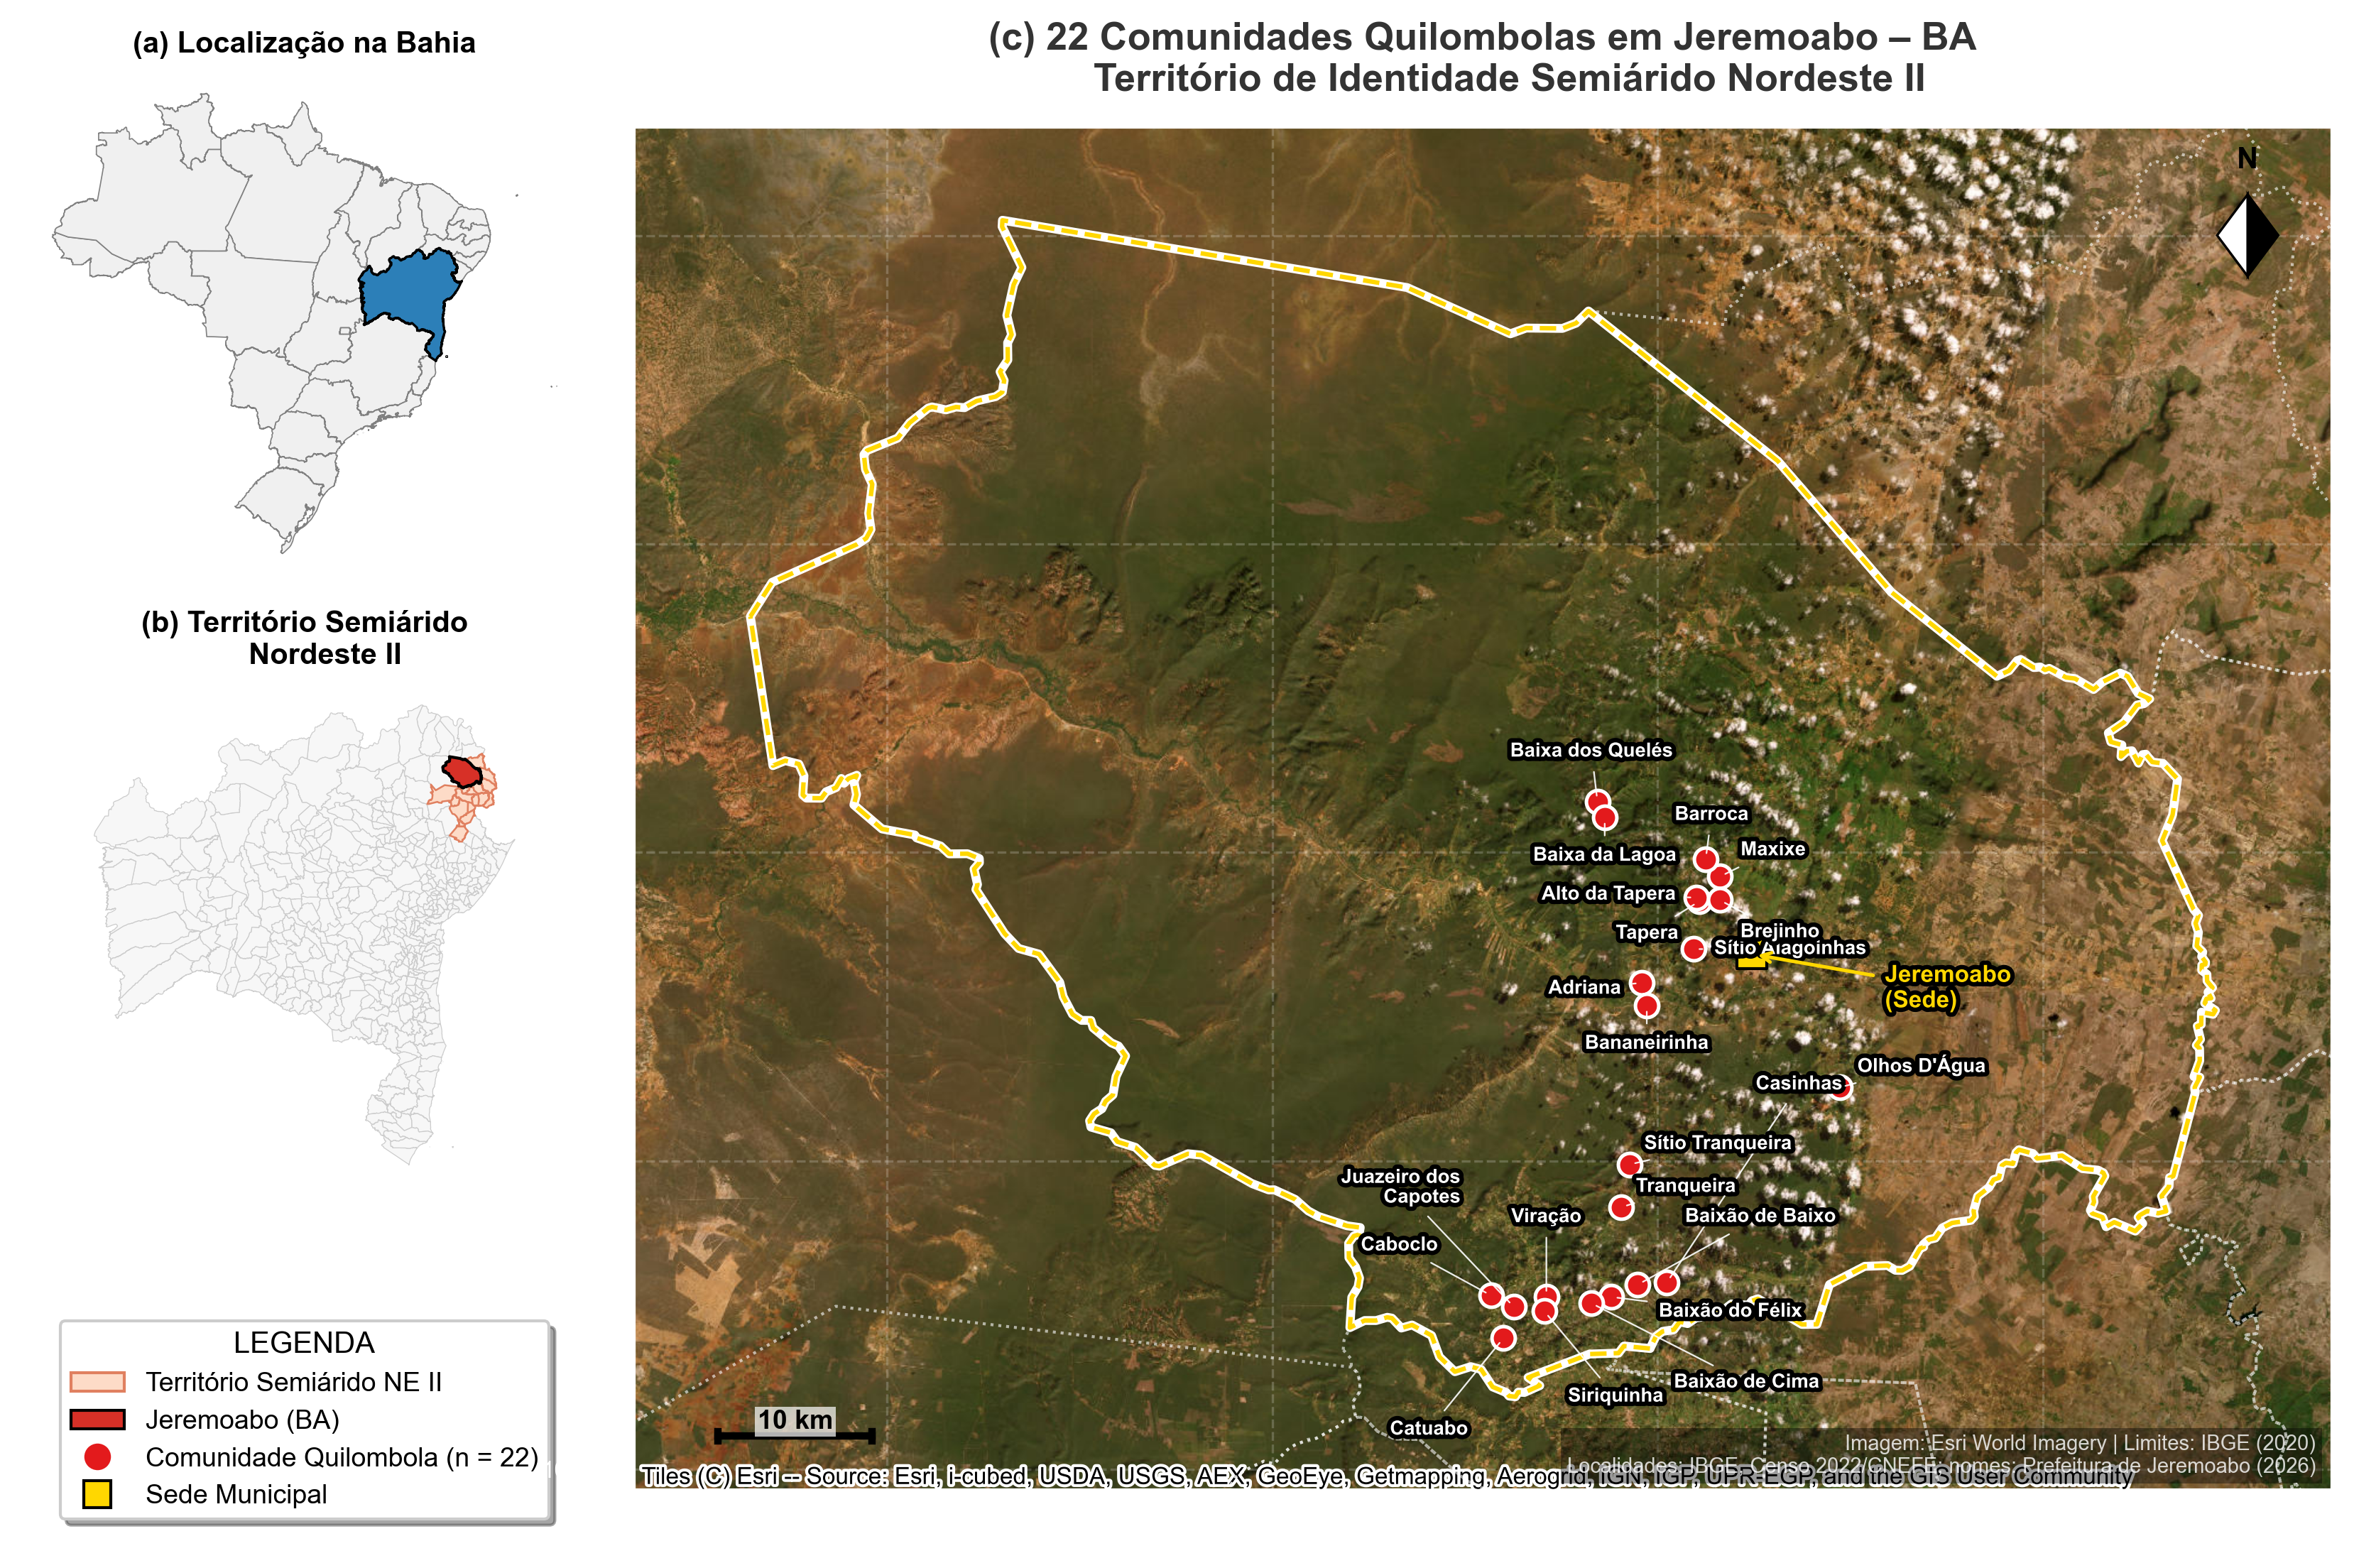
\includegraphics[width=\textwidth]{FIGURAS/territorio_satelite.png}
\fonte{\textbf{Elaborado pelos autores} (2026), sobre limites municipais do IBGE (2020) e imagem Esri World Imagery, em SIRGAS 2000.}
\end{figure}

O conjunto de comunidades de destino reúne Baixão da Tranqueira, Casinhas, Viração, Ciriquinha, Baixão de Cima e Baixa dos Quelés. A base empírica que alimenta a adaptação provém das cinco primeiras, nas quais o diagnóstico participativo foi conduzido entre agosto e setembro de 2026 por meio de entrevistas semiestruturadas abertas, assembleias de pactuação, rodas intergeracionais e percursos de reconhecimento territorial conduzidos por mestres e mestras de saberes. A coleta em Baixa dos Quelés está prevista para etapa subsequente, sob o mesmo protocolo, e o instrumento adaptado será aplicado nas seis comunidades.

\subsection{Operacionalização das Dimensões a partir do Questionário WOCAT}

O questionário WOCAT para Tecnologias de gestão sustentável da terra apresenta arquitetura modular em sete seções \cite{Liniger2019}, das quais seis oferecem conteúdo operacionalizável para as oito dimensões de vulnerabilidade biocultural ($V_1$--$V_8$) adotadas. A seção de definição, especificações técnicas e classificação de medidas alimenta a erosão intergeracional e migração ($V_1$) e o status de documentação ($V_3$). A seção de uso da terra, degradação e função protetora fornece indicadores para a complexidade e singularidade biocultural ($V_2$). A seção de investimentos e fluxos econômicos contribui para a integração ao mercado ($V_7$). 

A seção de clima, topografia, solos e características dos usuários contribui para $V_2$, para a vulnerabilidade jurídica e fundiária ($V_4$) e para a exposição climática ($V_8$). A seção de impactos socioculturais, ecológicos e institucionais sustenta $V_1$, $V_2$, $V_3$, a organização social e governança ($V_5$), a vitalidade linguística ($V_6$) e $V_7$. A seção de referências complementa $V_3$ ao indicar a existência de publicações e registros formais, ao passo que a seção cadastral foi tratada como contexto descritivo.

A análise concentrou-se nas seções de definição, uso da terra, ambiente natural e impactos do questionário WOCAT, que contêm os campos avaliativos mais sensíveis à equivalência cultural, e utilizou as seções de insumos e custos e de referências do mesmo instrumento como fontes complementares para integração ao mercado e status de documentação. A Tabela~\ref{tab:wocat_dimensoes} explicita a correspondência analítica entre os módulos do instrumento e as oito dimensões, utilizada para confrontar os achados territoriais com a cobertura oferecida pelo WOCAT-SLM.

Essa correspondência localiza, no núcleo do instrumento, os campos que sustentam cada dimensão, e o confronto com o material de campo define quais delas o núcleo registra sem perda. O WOCAT-SLM foi concebido para documentar tecnologias de conservação do solo e da água em escala comparável entre países \cite{Liniger2019,Schwilch2011}, e sua arquitetura organiza-se em torno de atributos biofísicos, técnicos e econômicos da prática. A vitalidade da terminologia vernacular, a continuidade da transmissão entre gerações e a governança do acervo probatório distribuem-se, nessa arquitetura, entre subitens de impacto sociocultural e de referências documentais, e é essa dispersão que o módulo suplementar reorganiza.

\begin{table}[H]
\centering
\caption{Mapeamento entre seções do questionário WOCAT-SLM, dimensões de vulnerabilidade biocultural ($V_1$--$V_8$) e variáveis-chave para a análise territorial.}
\label{tab:wocat_dimensoes}
\small
\begin{tabular}{p{1cm}p{2.8cm}p{4cm}p{5cm}}
\toprule
\textbf{Dim.} & \textbf{Denominação} & \textbf{Seções WOCAT de origem} & \textbf{Variáveis-chave deriváveis} \\
\midrule
$V_1$ & Erosão Intergeracional e Migração \cite{ReyesGarcia2013evidence,GomezBaggethun2013,TangGavin2016} & §2 Descrição; §6.1 Impactos socioculturais & Proporção de jovens praticantes, taxa de transmissão ativa, significado ritual vinculado à prática, emigração juvenil, aculturação, oportunidades culturais de aprendizado \\
\addlinespace
$V_2$ & Complexidade e Singularidade Biocultural \cite{Maffi2001,Pretty2009,FernandezLlamazares2021,Zimmerer2018} & §3 Classificação; §5 Ambiente natural; §6.1 Impactos ecológicos & Agrobiodiversidade (Shannon $H'$, Simpson), riqueza de variedades locais, $\beta$-diversidade de práticas, endemismo de variedades, interações solo-planta codificadas \\
\addlinespace
$V_3$ & Status de Documentação \cite{Maina2012,Poorna2014,Balogun2021} & §2 Descrição; §6.5 Adoção; §7 Referências & Número de saberes com registro formal, completude de fichas técnicas, taxa de digitalização de acervos \\
\addlinespace
$V_4$ & Vulnerabilidade Jurídica e Fundiária \cite{Dutfield2004,Cottier2004,BavikatteRobinson2011} & §5.6 Características dos usuários; §5.8 Propriedade & Mecanismos formais de proteção (IG, marca coletiva, registro IPHAN), existência de protocolo comunitário, regime fundiário, direitos de uso \\
\addlinespace
$V_5$ & Organização Social e Governança \cite{Berkes2004,OlssonFolkeBerkes2004,Folke2004} & §5.9 Infraestrutura; §6.1 Instituições comunitárias; §6.5 Adoção & Mestres de saberes ativos, frequência de eventos de transmissão, redes de cooperação, capital social, equidade de gênero \\
\addlinespace
$V_6$ & Vitalidade Linguística \cite{Moseley2010,Zent2014} & §2 Descrição (terminologia local); §6.1 Impactos socioculturais & Escala EGIDS, índice VITEK, proporção de falantes da língua vernacular, terminologia etnotaxonômica ativa \\
\addlinespace
$V_7$ & Integração ao Mercado \cite{Bellon2004,Brush2004} & §4 Insumos e Custos; §6.3 Impactos econômicos & Proporção de produção para venda, taxa de substituição de variedades crioulas, dependência de insumos externos \\
\addlinespace
$V_8$ & Exposição Climática \cite{Altieri2015,Dossou2022} & §5 Ambiente natural (clima); §6.1 Impactos ecológicos & SPI, frequência de eventos extremos, perda de safra por seca/excesso hídrico \\
\bottomrule
\end{tabular}
\end{table}

Os indicadores do questionário relativos à resposta da tecnologia à degradação da terra e à exposição a mudanças climáticas foram tratados como variáveis transversais. A resiliência edáfica e a exclusividade de práticas foram alocadas em $V_2$, enquanto a capacidade organizacional de resposta a perturbações foi alocada em $V_5$. Essa alocação manteve o modelo de oito dimensões derivado da síntese de evidências que precedeu este estudo.

% ============================================================
% FASE 1: ENTRADA EM CAMPO E DIAGNÓSTICO PARTICIPATIVO FORMATIVO
% ============================================================

\subsection{Confronto entre as Categorias Territoriais e os Campos do Questionário}

Cada entrada do guia de códigos foi comparada aos campos da seção do módulo de Tecnologias associada à respectiva dimensão de vulnerabilidade (Tabela~\ref{tab:wocat_dimensoes}). Uma planilha de rastreabilidade registrou sete elementos para cada confronto, compreendendo o código, a categoria axial, a dimensão correspondente, a seção e o campo do questionário, o tipo de desajuste, o ajuste proposto e o trecho de transcrição que sustentou o registro. Esses elementos permitem auditar cada especificação até a fala de origem \cite{Gioia2013}.

Um desajuste foi declarado quando nenhum campo do questionário admite o conteúdo da categoria, caso em que o registro é de ausência, ou quando existe campo pertinente cuja unidade de registro difere daquela com que os detentores operam a prática, caso em que o preenchimento fracionaria um arranjo que o território mantém unido. O desajuste também foi declarado quando o campo existe e a unidade é compatível, mas a categoria de resposta ou o termo empregado desloca o referente em relação ao vocabulário local, situação que a literatura de equivalência transcultural trata como falha de equivalência semântica ou experiencial \cite{Herdman1999,Beaton2000}.

A escolha entre ajustar campo existente e criar item suplementar seguiu regra de preservação da estrutura original. Sempre que algum campo do questionário pudesse acolher o conteúdo mediante reformulação de enunciado, categoria de resposta ou unidade de registro, a alteração foi especificada sobre esse campo, o que mantém a correspondência com a base internacional do WOCAT e preserva a comparabilidade dos registros. Item suplementar foi especificado apenas quando nenhum campo existente admitia o conteúdo sem perda de informação, e nesses casos a especificação indica a seção do questionário à qual o item se acopla.

O confronto foi conduzido sobre o corpus já codificado, sob o mesmo arranjo de autoria e de resolução de divergências adotado na codificação. Divergências entre categoria e campo que não se resolveram em especificação foram retidas na planilha como lacunas em aberto.

\subsection{Fase 2, em curso, Adaptação Transcultural do WOCAT-SLM}

A adaptação segue o modelo hierárquico de equivalência transcultural proposto por \citet{Herdman1999}, que discrimina as equivalências conceitual, de itens, semântica, operacional, de mensuração e funcional. O protocolo também observa os princípios de \citet{Guillemin1993} e \citet{Beaton2000}, com traduções independentes, retrotradução, revisão por comitê multidisciplinar e multicultural e pré-teste com a população-alvo. O procedimento busca preservar a comparabilidade internacional associada à dimensão \textit{etic} e incorporar as dimensões \textit{emic} relevantes ao contexto de aplicação.

\subsubsection{Etapa 1, Tradução Direta (Inglês $\rightarrow$ Português)}

% TODO: confirmar, para o dossiê de adaptação, se as versões T1 e T2 e os
% respectivos relatórios de decisão foram arquivados em separado.
A tradução direta do questionário WOCAT-SLM do inglês para o português brasileiro foi realizada e cobre as sete seções do instrumento. O procedimento seguiu a orientação de perfis contrastantes \cite{Beaton2000}, na qual uma das versões é produzida por profissional com formação em ciências agrárias, bilíngue e ciente dos objetivos do estudo, que privilegia a equivalência técnica, e a outra por profissional sem formação técnica na área, bilíngue e não informado dos objetivos, que privilegia a linguagem corrente. A divergência deliberada entre os perfis amplia a detecção de ambiguidades que uma tradução única tenderia a resolver silenciosamente.

\subsubsection{Etapa 2, Síntese das Traduções (T-12)}

A versão sintetizada em português brasileiro foi consolidada a partir das traduções diretas e está reproduzida na íntegra no Apêndice~\ref{app:wocat}. Esse texto compõe o instrumento de avaliação encaminhado ao comitê de especialistas. Cada um dos quarenta e oito itens das sete seções será julgado nas quatro dimensões de equivalência. Discrepâncias de tradução ainda não resolvidas foram mantidas em aberto para avaliação pelo comitê.

A correspondência entre o instrumento original em inglês \cite{Liniger2019} e a versão sintetizada foi conferida antes do encaminhamento ao comitê. Os quarenta e oito itens das seções 1 a 7 foram pareados sem omissão nem acréscimo. O comitê ainda avaliará a equivalência semântica de cada item.

\subsubsection{Etapa 3, Retrotradução (Português $\rightarrow$ Inglês)}

Dois retrotradutores independentes, nativos de língua inglesa ou com proficiência C2, sem conhecimento do original, traduzirão a versão sintetizada de volta para o inglês (BT1 e BT2). As retrotraduções serão comparadas com o instrumento original item a item, e as divergências que indicarem perda de significado retornarão à síntese antes do julgamento pelo comitê.

\subsubsection{Etapa 4, Comitê de Especialistas}

O comitê multidisciplinar será composto por 5 a 7 membros, incluindo mestres de saberes quilombolas (1 a 2 agricultores com experiência mínima de 20 anos), pesquisadores em agroecologia e etnoecologia (1 a 2 doutores com experiência participativa), especialistas em psicometria e adaptação transcultural (1) e gestores de PI e extensionistas (1 a 2).

A inclusão de mestres de saberes como membros plenos fundamenta-se no princípio de soberania epistêmica \cite{Santos2007} e nas diretrizes ITC \cite{ITC2017}.

O comitê avaliará cada item nas dimensões de equivalência semântica, idiomática, experiencial e conceitual, mediante escala de quatro pontos. O Índice de Validade de Conteúdo será calculado pela equação seguinte.

\begin{equation}
IVC_{item} = \frac{\text{nº de avaliadores que atribuíram 3 ou 4}}{\text{nº total de avaliadores}}
\end{equation}

Serão aceitos os itens que alcançarem $IVC \geq 0{,}80$, retornarão para revisão os situados no intervalo $0{,}60 \leq IVC < 0{,}80$ e serão reformulados ou excluídos aqueles com $IVC < 0{,}60$. A concordância interavaliadores será aferida por kappa de Fleiss \cite{Fleiss1971}. O instrumento de avaliação já se encontra construído e reúne os quarenta e oito itens das seções 1 a 7 da versão traduzida, dispostos por seção, com uma coluna por dimensão de equivalência, campo próprio para a redação alternativa proposta pelo avaliador e uma segunda via contendo o texto integral de cada item para consulta durante o julgamento. O comitê também identificará lacunas culturais e proporá itens suplementares.

\subsubsection{Etapa 5, Pré-Teste}

A versão pré-final será aplicada a 10--15 agricultores quilombolas de Jeremoabo (BA), selecionados por amostragem intencional com variabilidade em idade, gênero, escolaridade e sistema produtivo. A aplicação ocorrerá em formato de entrevista assistida. Ao término de cada seção, um debriefing cognitivo \cite{Willis2005} examinará a compreensão do enunciado, a adequação das alternativas linguísticas e a pertinência experiencial do item.

Serão registrados a taxa de compreensão por item, com limiar operacional de 85\%, a taxa de não resposta, com teto de 15\%, o tempo de aplicação e a distribuição das respostas, esta última destinada a detectar efeitos de teto e de piso.

\subsubsection{Etapa 6, Consolidação}

A versão final do WOCAT-SLM-QBR será consolidada em dossiê de adaptação que reúne as versões T1, T2, T-12, BT1 e BT2, as atas do comitê, os dados do pré-teste e o manual de aplicação, e será encaminhada ao WOCAT Secretariat.

\subsubsection{Etapa 7, Validação do Instrumento Adaptado}

A validação do instrumento WOCAT-SLM-QBR seguirá o modelo tripartite descrito no \textit{Standards for Educational and Psychological Testing} \cite{Association2018}, adaptado ao contexto de instrumentos de avaliação socioecológica.

A evidência de conteúdo será aferida pelo IVC e pelo kappa de Fleiss obtidos na avaliação do comitê, complementados pela taxa de compreensão apurada no pré-teste, eliminando-se os itens com $IVC < 0{,}60$ e devolvendo-se ao comitê aqueles situados entre $0{,}60$ e $0{,}80$. A evidência de estrutura interna dependerá de análise fatorial confirmatória conduzida após a aplicação do instrumento adaptado, destinada a verificar o ajuste do modelo de mensuração às oito dimensões teóricas, com avaliação dos índices CFI, TLI e RMSEA e da fidedignidade composta por dimensão.

A evidência baseada em relações com variáveis externas será obtida pela correlação entre as pontuações do instrumento e indicadores independentes disponíveis para o território, entre os quais índices de agrobiodiversidade, cobertura fundiária e indicadores socioeconômicos municipais, de modo a examinar validade convergente e discriminante. A evidência derivada do padrão de respostas resultará da inspeção das distribuições por item quanto a efeitos de piso e de teto, adotando-se 15\% em categoria extrema como limiar de alerta, e quanto a curtose e assimetria, submetendo-se a reavaliação qualitativa os itens com distribuição degenerada.

As análises de AFC e fidedignidade serão conduzidas em R versão 4.5.1 \cite{RCore2024}, empregando o pacote \texttt{lavaan} com estimador WLSMV para dados ordinais \cite{Sellbom2019FactorRecommendations} e o pacote \texttt{semTools} para cômputo de $\omega$ e $AVE$. Os resultados determinarão se o instrumento dispõe de evidências psicométricas suficientes para as etapas subsequentes de modelagem fuzzy.

% ============================================================
% FASE 3 (PLANEJADA): ELICITAÇÃO DELPHI
% ============================================================

\subsection{Fase 3, planejada, Elicitação Estruturada via Protocolo Delphi}

\subsubsection{Composição do Painel}

O painel será composto por 10 a 15 participantes selecionados por amostragem intencional \cite{Patton2015}, buscando heterogeneidade controlada entre quatro categorias de participantes, que compreendem mestres de saberes quilombolas (2 a 3 agricultores reconhecidos por suas comunidades, com experiência mínima de 20 anos), pesquisadores acadêmicos (3 a 4 doutores em agroecologia, etnoecologia, PI ou gestão da inovação), técnicos extensionistas (2 a 3, com experiência mínima de 5 anos em assessoria a comunidades tradicionais) e gestores de PI e bioeconomia (2 a 3, vinculados a NITs, SEBRAE, INPI ou secretarias territoriais).

A elegibilidade exigirá experiência mínima de cinco anos na área de atuação, reconhecimento pela comunidade epistêmica ou territorial de referência e disponibilidade para participar de três rodadas ao longo de quatro meses. A inclusão de mestres de saberes como especialistas de pleno direito é fundamentada em \cite{Santos2007,Beaton2000}.

\subsubsection{Estrutura das Rodadas}

A primeira rodada operará em regime aberto e solicitará ao painel variáveis relevantes para avaliar a vulnerabilidade e a salvaguarda dos sistemas agrícolas tradicionais. As respostas serão organizadas segundo as oito dimensões de vulnerabilidade biocultural apresentadas na Tabela~\ref{tab:wocat_dimensoes}. Os mestres de saberes participarão em formato assistido, com registro oral transcrito, para que a escrita não constitua barreira de participação. As respostas serão agrupadas semanticamente e as duplicidades serão eliminadas.

A segunda rodada submeterá a lista consolidada à avaliação da relevância, clareza e operacionalidade de cada variável em escala Likert de cinco pontos. Serão calculados a mediana, o intervalo interquartil, o coeficiente de variação e a frequência de respostas extremas. Na terceira rodada, o painel receberá as medianas, a distribuição das respostas e o posicionamento individual anonimizado. A conjunção de $IQR \leq 1{,}0$ e $Md \geq 4{,}0$ definirá o consenso operacional, e as variáveis abaixo desse patamar serão encaminhadas à análise qualitativa complementar.

\subsubsection{Análise Estatística do Consenso}

A análise estatística do consenso envolverá o cálculo de mediana e intervalo interquartil por variável e por rodada, avaliando-se a redução progressiva do intervalo e adotando-se $IQR \leq 1$ em escala de cinco pontos como limiar operacional de convergência \cite{VonDerGracht2012}. O coeficiente de concordância de Kendall ($W$) será empregado como indicador de consenso, adotando $W \geq 0{,}70$ como consenso forte e $0{,}50 \leq W < 0{,}70$ como moderado \cite{Schmidt2014}. O Coeficiente de Validade de Conteúdo (CVC) seguirá critério $CVC \geq 0{,}80$ \cite{Hernandez-Nieto2002}. A taxa de estabilidade entre as rodadas 2 e 3 será aferida pelo percentual de painelistas com ajuste $\pm 1$ ponto, adotando-se limiar mínimo de 70\% de painelistas estáveis como critério de convergência suficiente \cite{Dajani1979}. O teste de Friedman ($\alpha = 0{,}05$) com \textit{post-hoc} de Dunn será aplicado quando aplicável.

\subsubsection{Critérios de Parada e Tratamento de Variáveis sem Consenso}
\label{sec:delphi_parada}

O protocolo Delphi adotará critérios de parada explícitos para assegurar rigor no encerramento das rodadas e tratamento sistemático de variáveis que não atinjam consenso. O processo será encerrado após a terceira rodada independentemente do nível de consenso atingido, conforme prática recomendada na literatura \cite{Diamond2014}. Variáveis que ao final da Rodada~3 satisfizerem simultaneamente $IQR \leq 1{,}0$, $Md \geq 4{,}0$ e $CVC \geq 0{,}80$ serão classificadas como ``consenso atingido'' e incorporadas ao instrumento ISB. Variáveis com $W \geq 0{,}50$ mas $IQR > 1{,}0$ serão classificadas como ``consenso parcial'' e retidas no instrumento com sinalização explícita de incerteza nos metadados, sendo submetidas a análise qualitativa complementar mediante triangulação com as entrevistas semiestruturadas.

Variáveis com $W < 0{,}50$ e $IQR > 1{,}5$ serão classificadas como ``sem consenso'' e excluídas do ISB, permanecendo documentadas como candidatas para reavaliação em rodadas futuras caso novas evidências justifiquem sua reinclusão. A estabilidade entre rodadas será considerada insuficiente quando menos de 70\% dos painelistas mantiverem ajuste $\pm 1$ ponto entre R2 e R3 para uma variável específica, caso em que a variável será reclassificada como ``consenso instável'' mesmo que os limiares de $IQR$ e $Md$ tenham sido satisfeitos.

Todas as análises serão conduzidas em ambiente R versão 4.5.1 \cite{RCore2024}, empregando o pacote \texttt{irr} para cômputo de $W$ de Kendall e coeficientes de concordância, o pacote \texttt{PMCMRplus} para o teste de Friedman com comparações \textit{post hoc} de Dunn ajustadas por Bonferroni e funções nativas do pacote \texttt{stats} para estatísticas descritivas, enquanto o $CVC$ será calculado via rotina própria implementada conforme algoritmo de \citet{Hernandez-Nieto2002}.

Para a H3(b), a convergência interna do Delphi será descrita pela variação do IQR e do coeficiente~$W$ de Kendall entre a Rodada~1 aberta e as Rodadas~2 e~3 estruturadas. Como as rodadas são sequenciais e incluem realimentação, essa comparação não constitui teste direto de superioridade entre métodos.

\subsection{Modalidade de Aplicação do Instrumento Adaptado}

O léxico etnotaxonômico levantado nas oficinas alimentará diretamente a síntese das traduções e a avaliação pelo comitê de especialistas, fornecendo o vocabulário vernacular contra o qual a equivalência semântica e experiencial de cada item será julgada. O inventário de tecnologias candidatas documentado na Fase 1 constituirá o objeto concreto de aplicação no pré-teste, o que evita que o debriefing cognitivo opere sobre situações hipotéticas. As ordenações de impacto e urgência produzidas pela matriz de priorização por pares serão apresentadas ao painel como insumo de campo da Rodada~1 do Delphi, ancorando a enumeração de variáveis candidatas em práticas efetivamente observadas no território.

Concluída a consolidação do WOCAT-SLM-QBR, a oficina participativa permanecerá como modalidade primária de aplicação do instrumento. Essa escolha decorre da estrutura de distribuição do conhecimento nos SSAT quilombolas, na qual o manejo é operado sob lógica coletiva \cite{Ostrom1990,Toledo2008}, de forma que a unidade de resposta pertinente é o coletivo de usuários da terra. 

A entrevista domiciliar dirigida opera como modalidade complementar e subordinada, acionada exclusivamente para os campos ancorados em memória longa cujos detentores não comparecem à plenária por restrição de mobilidade ou não expõem determinado conteúdo em ambiente coletivo, condição documentada na entrevista exploratória que abriu esta fase. Essa complementaridade não reintroduz o indivíduo como unidade de resposta, pois os registros assim obtidos retornam à plenária para validação coletiva sempre que o detentor autorize, e permanecem sinalizados no dossiê quando a autorização não for concedida.

% ============================================================
% FASE 2 (PLANEJADA): ADAPTAÇÃO TRANSCULTURAL
% ============================================================
% TODO — NÃO COMPILADO: concluir tradução, síntese, retrotradução, comitê,
% pré-teste e validação de conteúdo antes de transformar este material em artigo.
% O Delphi deve ser reportado somente com base completa das rodadas e métricas.

\subsection{Triangulação por Entrevistas Semiestruturadas}

A série de entrevistas semiestruturadas abertas iniciada na Fase 1 prosseguirá por amostragem teórica com agricultores quilombolas de Jeremoabo. O roteiro incorporará a percepção sobre as variáveis levadas ao Delphi, eventuais dimensões não contempladas, a adequação da linguagem e a hierarquização espontânea de urgências, sem abandonar o formato aberto. A saturação teórica das categorias centrais determinará o encerramento \cite{Glaser1967}. Estimam-se oito a dez entrevistas adicionais com base na densidade das categorias já constituídas.

As entrevistas serão gravadas em áudio, transcritas integralmente, conferidas quanto à atribuição de turnos e ao vocabulário vernacular e submetidas aos ciclos de codificação adotados na Fase 1 \cite{CorbinStrauss2015,Saldana2021}. Dois pesquisadores conduzirão a codificação de forma independente, com kappa de Cohen $\geq 0{,}60$ \cite{Landis1977}. Uma matriz relacionará as variáveis validadas pelo painel às categorias axiais emergentes. A análise temática \cite{Braun2006} será utilizada apenas na sumarização descritiva.

\subsection{Aspectos Éticos}

Este estudo foi aprovado pelo Comitê de Ética em Pesquisa da Universidade Federal de Sergipe (CEP-UFS), sob o CAAE~96596826.9.0000.5546, em conformidade com as Resoluções CNS nº~466/2012 e nº~510/2016. Todos os participantes forneceram consentimento livre, prévio e informado antes de qualquer procedimento de coleta. Nas entrevistas gravadas, a autorização para registro em áudio foi obtida de forma destacada do consentimento para participação, e o áudio foi eliminado após a transcrição integral e a conferência da transcrição, permanecendo no acervo apenas o texto transcrito sob identificação por código. A anuência coletiva para a atividade participativa de 19 de agosto de 2026 foi formalizada em assembleia comunitária.

% TODO: confirmar os procedimentos de titularidade, divulgação
% cartográfica, coautoria do instrumento e devolutiva antes de reportá-los como
% práticas executadas nas oficinas, na adaptação transcultural ou no Delphi.


O protocolo prevê o reconhecimento dos mestres de saberes integrantes do comitê de adaptação transcultural como coautores do instrumento WOCAT-SLM-QBR. Também prevê o tratamento de dados sensíveis e conhecimentos tradicionais conforme o Protocolo de Nagoia e a Lei nº~13.123/2015, além da devolutiva dos resultados às comunidades.

\section{Resultados e Discussão}

\subsection{Cobertura do Núcleo e Delimitação do Bloco Suplementar}

A auditoria confrontou cada um dos vinte e dois códigos do guia produzido no diagnóstico participativo com o texto integral dos quarenta e oito itens das seções 1 a 7 do módulo de Tecnologias. Quatro códigos encontraram no núcleo campo capaz de registrá-los sem perda, dez não encontraram campo pertinente e oito encontraram campo que acolhe parte do conteúdo e deixa a parte restante sem registro. A Tabela~\ref{tab:mapeamento_codigos} apresenta a atribuição resultante, com o campo do núcleo e o módulo do bloco suplementar indicados separadamente para cada código.

Os quatro códigos integralmente cobertos pelo núcleo descrevem atributos que o instrumento foi construído para documentar. O portfólio de microatividades e a captação e reserva de água de chuva são arranjos técnicos de uso da terra e de manejo hídrico, o acesso desigual à infraestrutura hídrica corresponde ao campo de infraestrutura disponível aos usuários e o escoamento operado por mulheres cabe nos campos de destino da produção. A permanência desses códigos no núcleo preserva a comparabilidade internacional do registro correspondente.

A auditoria também corrigiu atribuições feitas por aproximação na primeira versão do guia. A seção 6.5 do questionário havia sido associada aos códigos de transmissão, e o exame do enunciado mostrou que esse campo registra a proporção de usuários que adotaram a tecnologia documentada, construto distinto da dinâmica demográfica pela qual o saber passa de uma geração a outra. Os quatro códigos de transmissão foram realocados ao bloco suplementar, e a seção 6.5 permaneceu vinculada ao que de fato mede.

Os dezoito códigos restantes originaram o bloco suplementar, organizado como seção 9 do WOCAT-SLM-QBR e composto por nove módulos apresentados na Tabela~\ref{tab:modulos_secao9}. O módulo de singularidade territorial não recebeu código do guia, porque seu conteúdo provém da leitura da topossequência e do inventário de recursos, registros de observação que a codificação das entrevistas não produz, e foi mantido no bloco por corresponder a campo exigido pelos demais instrumentos do diagnóstico.

Os nove módulos foram redigidos em cinquenta itens, reproduzidos na íntegra no Apêndice~\ref{app:wocat}, e distribuem-se de modo desigual entre as dimensões, com onze itens na transmissão intergeracional e ritual, oito na governança comunitária, seis na proteção jurídica e propriedade intelectual, cinco na agrobiodiversidade e etnotaxonomia, cinco no déficit documental, quatro na singularidade territorial, quatro na vitalidade linguística, quatro na integração ao mercado e três na exposição climática. A concentração no primeiro módulo acompanha o número de códigos que a ele remetem e a variedade de mecanismos pelos quais a descontinuidade da transmissão se manifestou no corpus.

Os itens organizam-se em quatro camadas de aplicação, definidas pelo tipo de informante e de registro que cada uma exige. A primeira reúne o autorrelato do agricultor e da liderança comunitária, a segunda depende de inventário conduzido em campo pelo agricultor junto do pesquisador, a terceira é preenchida pelo compilador a partir de auditoria documental e jurídico-institucional e a quarta agrega os módulos focais de vitalidade linguística, integração ao mercado e exposição climática. Essa estratificação determina em que momento do trabalho de campo cada item pode ser respondido e evita que a oficina participativa seja interrompida por perguntas que dependem de consulta a arquivo.

Três itens não derivam de um código isolado e sim das especificações produzidas pelo confronto entre as categorias e os campos existentes. O item que documenta a composição do portfólio familiar de atividades registra o arranjo que o instrumento de origem fracionaria em fichas separadas; o item que registra as espécies retiradas do portfólio opera em dupla referência temporal, com a área anterior ao abandono ao lado da atual; e o item de desagregação da resposta por gênero e geração é de controle de aplicação, preenchido pelo compilador, e retém a divergência entre os estratos sem conciliá-la. A quarta especificação, relativa à pactuação, incorporou-se ao módulo de governança como item que registra quantas entidades reivindicam representar a comunidade.

\begin{table}[H]
\centering
\caption{Módulos do bloco suplementar (seção 9) do WOCAT-SLM-QBR, com o conteúdo que cada um registra e as dimensões de vulnerabilidade biocultural a que se vincula.}
\label{tab:modulos_secao9}
\small
\setlength{\tabcolsep}{4pt}
\begin{tabular}{p{0.9cm}p{3.6cm}p{6.6cm}p{1.9cm}}
\toprule
\textbf{Mód.} & \textbf{Denominação} & \textbf{Conteúdo registrado} & \textbf{Dim.} \\
\midrule
§9.1 & Transmissão intergeracional e ritual & Regime demográfico do trabalho familiar, permanência dos aprendizes no território, calendário festivo acoplado ao ciclo produtivo e cronologia da ocupação por gerações nomeadas & $V_1$ \\
\addlinespace
§9.2 & Governança comunitária & Entidades que reivindicam representação, continuidade institucional e administração da infraestrutura coletiva de beneficiamento & $V_5$ \\
\addlinespace
§9.3 & Agrobiodiversidade e etnotaxonomia & Variedades crioulas nomeadas, critério local de seleção e guarda de semente e repertório de espécies de uso medicinal com indicação declarada & $V_2$ \\
\addlinespace
§9.4 & Singularidade territorial & Posição das parcelas na topossequência, classes locais de solo e recursos hídricos de uso comum que delimitam a unidade documentada & $V_2$, $V_4$ \\
\addlinespace
§9.5 & Déficit documental & Custódia e suporte físico do acervo probatório, alterações toponímicas e registros formais existentes sobre a comunidade & $V_3$ \\
\addlinespace
§9.6 & Proteção jurídica e propriedade intelectual & Estágio da certificação, regime de posse interno ao território coletivo e episódios declarados de expropriação da safra & $V_4$ \\
\addlinespace
§9.7 & Vitalidade linguística & Terminologia vernacular de manejo em uso corrente, repertório musical e coreográfico e etnônimos suprimidos ou substituídos & $V_6$ \\
\addlinespace
§9.8 & Integração ao mercado & Elos não monetários de circulação, remuneração em espécie pelo uso de infraestrutura e composição da renda com transferências & $V_7$ \\
\addlinespace
§9.9 & Exposição climática & Espécies retiradas do portfólio por restrição hídrica, com registro da situação anterior ao abandono & $V_8$ \\
\bottomrule
\end{tabular}
\fonte{\textbf{Elaborado pelos autores} (2026).}
\end{table}

\begin{table}[H]
\centering
\caption{Atribuição dos vinte e dois códigos do guia de codificação aos campos do núcleo do WOCAT-SLM e aos módulos do bloco suplementar do WOCAT-SLM-QBR.}
\label{tab:mapeamento_codigos}
\footnotesize
\setlength{\tabcolsep}{4pt}
\begin{tabular}{p{1.9cm}p{5.0cm}p{1.3cm}p{2.6cm}p{2.4cm}}
\toprule
\textbf{Código} & \textbf{Categoria registrada} & \textbf{Dim.} & \textbf{Campo do núcleo} & \textbf{Módulo §9} \\
\midrule
TRA-DEM & Regime demográfico do trabalho familiar & $V_1$ & --- & §9.1 \\
TRA-MIG & Migração juvenil com recusa do trabalho na terra & $V_1$ & --- & §9.1 \\
TRA-REP & Substituição do repertório cultural & $V_1$, $V_6$ & --- & §9.1; §9.7 \\
TRA-PER & Transmissão condicionada à permanência & $V_6$ & --- & §9.1; §9.7 \\
\addlinespace
MAN-PORT & Portfólio de microatividades & $V_2$ & §2.3; §3.1 & --- \\
MAN-SEM & Semente crioula como gestão de risco & $V_2$, $V_8$ & §2.3 & §9.3 \\
MAN-CONT & Contração do portfólio de espécies & $V_8$ & §4.2--4.5 & §9.9 \\
MAN-FEST & Calendário festivo acoplado ao ciclo produtivo & $V_2$, $V_8$ & §2.3; §4.2--4.5 & §9.1 \\
MAN-BEN & Estado da infraestrutura coletiva de beneficiamento & $V_2$, $V_5$ & §4.2--4.5 & §9.2 \\
MAN-CAPT & Captação e reserva de água de chuva & $V_2$, $V_8$ & §3.4; §3.5 & --- \\
MAN-FARM & Farmacopeia local acoplada ao manejo & $V_2$, $V_6$ & --- & §9.3 \\
MAN-FIB & Beneficiamento de fibra e tecnologia de substituição & $V_2$, $V_7$ & §4.4--4.7 & §9.8 \\
\addlinespace
PRO-CUST & Custódia distribuída do acervo probatório & $V_3$ & --- & §9.5 \\
PRO-REC & Reconhecimento incompleto & $V_3$, $V_4$ & --- & §9.5; §9.6 \\
\addlinespace
TER-EXP & Expropriação histórica da safra & $V_4$ & --- & §9.6 \\
TER-CRON & Cronologia por gerações nomeadas & $V_1$, $V_3$ & §2.5 & §9.1 \\
TER-REDE & Rede de parentesco entre povoados & $V_1$, $V_4$ & §2.5 & §9.1; §9.6 \\
TER-TOPO & Alteração toponímica e etnônimo suprimido & $V_3$, $V_6$ & --- & §9.5; §9.7 \\
\addlinespace
INF-AGUA & Acesso desigual à infraestrutura hídrica & $V_5$, $V_8$ & §3.4; §5.9 & --- \\
GOV-INT & Intermitência institucional & $V_5$ & --- & §9.2 \\
\addlinespace
CIR-MUL & Escoamento operado por mulheres & $V_7$ & §4.6--4.7 & --- \\
CIR-REN & Renda composta e autoconsumo & $V_7$ & §4.6--4.7 & §9.8 \\
\bottomrule
\end{tabular}
\fonte{\textbf{Elaborado pelos autores} (2026).}
\end{table}

A distribuição dos códigos entre núcleo e bloco suplementar mostra que a insuficiência do instrumento de origem não se distribui de modo uniforme pelas oito dimensões. As dimensões de natureza técnica e econômica, que descrevem o arranjo produtivo e a circulação da produção, encontram no núcleo campos que as registram com ajuste de enunciado. As dimensões que descrevem a continuidade da transmissão, a vitalidade da terminologia e a governança do acervo probatório concentram os códigos sem campo correspondente, o que é coerente com a finalidade para a qual o WOCAT-SLM foi construído \cite{Liniger2019,Schwilch2011}. O acréscimo especificado incide, portanto, sobre a parte do objeto que o instrumento internacional não se propôs a documentar, e não sobre a parte que ele documenta bem.

Esse resultado situa o caso na hierarquia de equivalências de \citet{Herdman1999}. Os oito códigos de atribuição mista correspondem a itens cuja equivalência conceitual se sustenta e cuja equivalência de itens exige complemento, situação que o protocolo de tradução resolve por reformulação de enunciado e por acréscimo de campo acoplado à seção de origem. Os dez códigos sem campo no núcleo correspondem a construtos ausentes do instrumento de origem, para os quais a tradução não tem objeto sobre o que operar, e cuja incorporação exige a redação de itens novos submetidos ao mesmo julgamento de equivalência conceitual e experiencial pelo comitê de especialistas \cite{Beaton2000}.

\subsection{Estado Corrente do Protocolo de Adaptação}

A tradução direta e a síntese das traduções foram concluídas para as sete seções do núcleo. A correspondência entre o instrumento original em inglês \cite{Liniger2019} e a versão sintetizada em português brasileiro foi conferida item a item antes do encaminhamento ao comitê, e os quarenta e oito itens foram pareados sem omissão nem acréscimo. A versão sintetizada está reproduzida na íntegra no Apêndice~\ref{app:wocat} e compõe o instrumento de avaliação submetido ao comitê de especialistas.

O instrumento de avaliação de conteúdo foi construído segundo o modelo de \citet{Beaton2000}, com julgamento de cada item nas equivalências semântica, idiomática, experiencial e conceitual em escala de quatro pontos, e apresenta o enunciado original em inglês ao lado da versão em português para que o especialista confronte as duas formulações. O índice de validade de conteúdo será calculado por item como a proporção de julgamentos nas duas categorias superiores, adotando-se o limiar de 0,80 para retenção direta e de 0,60 para reformulação, com descarte abaixo desse valor \cite{Hernandez-Nieto2002,Cassepp-Borges2010}. A concordância entre os especialistas será aferida pelo kappa de Fleiss \cite{Fleiss1971}, interpretado segundo os limiares de \citet{Landis1977}.

Os cinquenta itens do bloco suplementar estão redigidos e entram nesse mesmo instrumento de avaliação a partir da Etapa 4, uma vez que sua formulação decorre das categorias territoriais e não de um enunciado de origem a traduzir. O comitê julga, para esses itens, a equivalência conceitual e a experiencial, e o julgamento incide sobre a correspondência entre o enunciado proposto e a categoria elicitada em campo, cuja evidência consta da planilha de rastreabilidade que acompanha o dossiê de adaptação.

\subsection{Especificações de Adaptação sobre Campos Existentes}

O Diagnóstico participativo formativo produziu quatro especificações de adaptação, cada uma registrando o campo afetado do módulo de Tecnologias, o desajuste observado em campo e o ajuste correspondente. As especificações derivam da configuração documentada no território.

A unidade de registro do questionário é a prática de manejo isolada. O portfólio familiar de microatividades elicitado nas entrevistas mostrou que os agricultores operam essas práticas como arranjo único, e a especificação registrada prevê item suplementar que documente a composição do portfólio e o critério com que a família distribui trabalho e terra entre seus componentes.

O mesmo desajuste entre formato e prática reaparece no eixo temporal do instrumento, no qual o calendário sazonal admite uma única referência. O abandono do arroz e a retração do feijão, elicitados na entrevista com o informante-chave, mostraram que esse formato captura apenas a situação atual de um processo de abandono ainda em curso, e a especificação correspondente estabelece preenchimento em dupla referência, com a distribuição de operações anterior à saída das espécies registrada ao lado da atual.

A duplicação exigida no eixo temporal tem correspondência na esfera social do registro, que o questionário atribui a um respondente por unidade produtiva. As entrevistas mostraram que o escoamento da produção e a decisão sobre sementes se distribuem de modo desigual entre gêneros e gerações, e a especificação determina ordenações desagregadas para mulheres, jovens e mestres de saberes, com retenção das divergências abaixo do limiar de concordância.

A pluralidade que o instrumento passou a capturar entre gêneros e gerações reapareceu, no plano institucional, no protocolo de pactuação, que pressupunha uma entidade representativa por comunidade. O corpus documental registrou associações concorrentes na mesma comunidade e a obtenção de certificação por intermediação política \cite{Fernandes2013}, e o procedimento foi alterado ainda na Fase 1, passando a verificar quantas entidades reivindicam representação antes de cada oficina e a registrar a anuência de todas. A Tabela~\ref{tab:especificacoes} consolida o campo afetado, o desajuste observado, o ajuste correspondente e a evidência que sustenta cada especificação.

\begin{table}[H]
\centering
\caption{Especificações de adaptação do módulo de Tecnologias WOCAT-SLM produzidas na Fase 1, com campo afetado, desajuste observado, ajuste correspondente e evidência de origem.}
\label{tab:especificacoes}
\small
\setlength{\tabcolsep}{4pt}
\begin{tabular}{p{2.5cm}p{4.1cm}p{3.7cm}p{2.5cm}}
\toprule
\textbf{Campo afetado} & \textbf{Desajuste observado} & \textbf{Ajuste correspondente} & \textbf{Evidência} \\
\midrule
Unidade de registro (§2.3; §3.1) & O questionário registra a prática de manejo isolada, ao passo que cada unidade familiar opera três a quatro atividades como arranjo único & Item suplementar que documente a composição do portfólio e o critério de distribuição de trabalho e terra entre seus componentes & E2 \\
\addlinespace
Calendário sazonal (§2.3; §4.2--4.5) & Única referência temporal captura apenas a situação atual de um processo de abandono ainda em curso & Preenchimento em dupla referência, com a distribuição de operações anterior à saída das espécies registrada ao lado da atual & E1 \\
\addlinespace
Respondente (§5.6) & Registro atribuído a um respondente por unidade produtiva, com escoamento e decisão sobre sementes distribuídos de modo desigual entre gêneros e gerações & Ordenações desagregadas para mulheres, jovens e mestres de saberes, com retenção das divergências abaixo do limiar de concordância & E3 \\
\addlinespace
Pactuação (etapa pré-oficina) & Protocolo pressupunha uma entidade representativa por comunidade, com associações concorrentes e certificação por intermediação política no município & Verificação de quantas entidades reivindicam representação antes de cada oficina e registro da anuência de todas & \cite{Fernandes2013} \\
\bottomrule
\end{tabular}
\end{table}

As quatro especificações qualificam o desenho do instrumento, e a evidência que as sustenta permanece delimitada, uma vez que os resultados derivam de três entrevistas, de oficinas de reconhecimento territorial realizadas em quatro comunidades e de um corpus documental do mesmo município, e constituem categorias preliminares orientadas à construção do instrumento. A Fase 1 estabeleceu quais ajustes o instrumento exige, enquanto a mensuração da frequência dos fenômenos que os motivam cabe às etapas posteriores.


%%%%%%%%%%%%%%% AINDA A FAZER ESSA PARTE %%%%%%%%%%

\section{Desdobramentos Metodológicos e Produtos Esperados}

Esta seção descreve etapas ainda não executadas e não integra os resultados. Os produtos e os critérios indicados permanecem condicionados à execução dos respectivos procedimentos.


%%%   A SER DESENVOLVIDO %%%%%

\subsection{Produtos da Adaptação Transcultural}

O produto previsto é a versão WOCAT-SLM-QBR, condicionada a IVC global $\geq$~0,90 e kappa de Fleiss $\geq$~0,75. O dossiê reunirá relatórios T1/T2, retrotraduções, atas do comitê, planilhas do pré-teste e manual de aplicação. Sua utilidade em outros contextos de comunidades tradicionais brasileiras dependerá de avaliação específica.

O mapeamento examinará possíveis lacunas nas dimensões espiritual-ritual, de transmissão intergeracional por oralidade e de coletividade associada a bens comuns. Somente as lacunas sustentadas pelos dados serão convertidas em itens suplementares nas dimensões $V_1$--$V_8$ pertinentes. A análise testará se categorias \textit{etic} deslocam referentes locais quando aplicadas a ontologias distintas \cite{Herdman1999}, problema relacionado à vulnerabilidade documental dos sistemas de conhecimento indígena \cite{Maina2012,Balogun2021}.

\subsection{Produtos da Elicitação Delphi}

Prevê-se um conjunto validado de 20 a 30 variáveis linguísticas, acompanhadas de definições operacionais consensuadas e organizadas nas oito dimensões de vulnerabilidade biocultural ($V_1$--$V_8$) derivadas da meta-análise prévia. Cada variável disporá de ficha técnica contendo estatísticas descritivas ($Md$, $IQR$) e índices de consenso ($W$, $CVC$), com mapeamento para os indicadores do Índice de Salvaguarda Biocultural (ISB).

A evolução dos coeficientes de concordância entre a Rodada~1 aberta e as Rodadas~2--3 estruturadas será descrita em relação aos limiares de $W \geq 0,70$ e $CVC \geq 0,80$. Esse desenho sequencial não permite atribuir eventual convergência apenas à estruturação do método. A integração entre adaptação transcultural e elicitação Delphi será examinada à luz da gestão da inovação \cite{Tidd2005} e da economia de ativos intangíveis \cite{Lev2001}. Se validadas, as variáveis poderão apoiar a representação dos atributos VRIN e sua aplicação em processos de repartição de benefícios, certificação de produtos e proteção jurídica \cite{Belletti2015}.

\subsection{Contribuições Esperadas}

A articulação entre protocolo de adaptação e princípios ISO~30401 (Gestão do Conhecimento) pode oferecer contribuição teórica à literatura de gestão da propriedade intelectual em contextos comunitários. Ao documentar cada decisão com rastreabilidade, o dossiê de adaptação cria infraestrutura de metadados que atende simultaneamente requisitos de governança do conhecimento \cite{ISO30401} e demandas de proteção de conhecimentos tradicionais associados à biodiversidade, posicionando o estudo na interface entre psicometria transcultural e gestão estratégica de PI \cite{Teece1986,ISO56005}. No plano jurídico, essa cadeia responde às lacunas de proteção identificadas por \citet{Dutfield2004} e \citet{Cottier2004}, na medida em que o instrumento documentado e o consenso auditável podem instruir mecanismos \textit{sui generis} de proteção e protocolos bioculturais comunitários \cite{BavikatteRobinson2011,Nemoga2022,Robinson2014}.

Se o instrumento for validado, suas variáveis poderão alimentar as funções de pertinência e as regras de inferência de um sistema difuso do tipo Mamdani. A origem de cada variável do ISB será documentada para permitir o rastreamento entre WOCAT original $\rightarrow$ WOCAT-SLM-QBR $\rightarrow$ consenso Delphi $\rightarrow$ meta-análise $\rightarrow$ modelo fuzzy \cite{Costanza1997}. O manual registrará as decisões do protocolo integrado de adaptação e Delphi.

\section{Considerações Finais}

O protocolo de adaptação transcultural do módulo de Tecnologias do WOCAT-SLM para comunidades quilombolas do semiárido combina a equivalência item a item das sete seções do núcleo com a especificação de um bloco suplementar derivado de evidência territorial. A auditoria dos vinte e dois códigos do guia de codificação contra os quarenta e oito itens do núcleo estabeleceu a fronteira entre as duas operações, com quatro códigos integralmente cobertos pelo instrumento de origem, dez sem campo correspondente e oito de atribuição mista.

O bloco suplementar ficou constituído como seção 9 do WOCAT-SLM-QBR, com nove módulos e cinquenta itens que registram a transmissão intergeracional e ritual, a governança comunitária, a agrobiodiversidade e a etnotaxonomia, a singularidade territorial, o déficit documental, a proteção jurídica e a propriedade intelectual, a vitalidade linguística, a integração ao mercado e a exposição climática. O confronto entre as categorias territoriais e os campos existentes produziu, além desse bloco, quatro especificações de adaptação que incidem sobre a unidade de registro, o eixo temporal do calendário sazonal, a titularidade da resposta e o protocolo de pactuação.

A separação entre núcleo e bloco suplementar preserva a comparabilidade internacional dos registros produzidos nas seções que o WOCAT-SLM já cobre e concentra o acréscimo em parte identificada do instrumento, o que permite agregar os dados do território à base global sem que o conteúdo acrescentado se confunda com o conteúdo original. A rastreabilidade entre cada item proposto e a categoria elicitada em campo permite a um terceiro refazer o julgamento sobre a mesma base documental.

O alcance dos resultados aqui relatados corresponde ao estado do protocolo. A tradução direta e a síntese estão concluídas para as sete seções do núcleo, e a retrotradução, o julgamento por comitê de especialistas, o pré-teste e a validação de conteúdo compõem as etapas subsequentes. Os índices de validade de conteúdo, a concordância entre especialistas e as decisões de retenção, reformulação e descarte de itens serão reportados quando o comitê concluir o julgamento. A estrutura de nove módulos e a atribuição dos códigos constituem o produto desta etapa e o objeto sobre o qual esse julgamento incidirá.

%% ============================================================
%% Declarações de fim de artigo
%% ============================================================

\section*{Declaração de conformidade com diretriz de relato}

O relato deste estudo segue os Standards for Reporting Qualitative Research (SRQR), diretriz de vinte e um itens destinada a estudos qualitativos \cite{OBrien2014}. A diretriz foi adotada por se tratar de estudo metodológico que deriva de material qualitativo as decisões de adaptação do instrumento. A lista de verificação preenchida, com a localização de cada item no manuscrito, consta do Apêndice~\ref{app:srqr} e acompanha a submissão como material suplementar.

\section*{Declaração de conflito de interesses}

Os autores declaram não possuir conflitos de interesse financeiros ou relações pessoais conhecidas que possam ter influenciado o trabalho relatado neste artigo.

\section*{Disponibilidade de dados}

A versão sintetizada em português do módulo de Tecnologias, o instrumento de avaliação de conteúdo encaminhado ao comitê de especialistas e a planilha de rastreabilidade que vincula cada especificação ao campo afetado e à evidência de origem estão disponíveis mediante solicitação à autora correspondente. As transcrições integrais das entrevistas não são públicas, uma vez que o termo de consentimento assumiu compromisso de sigilo e as falas permitem identificação dos participantes em comunidades de pequeno porte.

% TODO: inserir o número do processo da bolsa CNPq e confirmar a quem foi
% concedida antes da submissão.
\section*{Agradecimentos}

Esta pesquisa foi realizada com apoio do Conselho Nacional de Desenvolvimento Científico e Tecnológico (CNPq), por meio de bolsa de doutorado concedida à primeira autora. Os autores agradecem às comunidades quilombolas de Baixão da Tranqueira, Casinhas, Viração, Ciriquinha e Baixão de Cima, cujas lideranças, mestres e mestras de saberes autorizaram a pesquisa em assembleia e conduziram o reconhecimento territorial.


\bibliographystyle{elsarticle-harv}
\bibliography{references}

\appendix
% ==========================================================
% APÊNDICE — Lista de verificação SRQR
% ==========================================================

\section{Lista de Verificação SRQR (Standards for Reporting Qualitative Research)}
\label{app:srqr}

\noindent Lista de vinte e um itens proposta por \cite{OBrien2014} para o relato de pesquisa qualitativa, com indicação da seção do manuscrito em que cada item é atendido.

{\footnotesize
\setlength{\tabcolsep}{3pt}
\begin{longtable}{p{3.6cm}p{4.6cm}p{5.6cm}}
\toprule
\textbf{Item} & \textbf{O que a diretriz requer} & \textbf{Onde é atendido} \\
\midrule
\endfirsthead
\toprule
\textbf{Item} & \textbf{O que a diretriz requer} & \textbf{Onde é atendido} \\
\midrule
\endhead
\midrule
\multicolumn{3}{r}{\footnotesize\textit{continua na próxima página}}\\
\endfoot
\bottomrule
\endlastfoot
\textbf{1} Título & Identifica o estudo como qualitativo e indica abordagem, método ou tipo de dado & Título do capítulo, que nomeia o diagnóstico participativo e as categorias derivadas \\
\addlinespace
\textbf{2} Resumo & Sintetiza problema, questão, abordagem, método, resultados e conclusões & Resumo e Abstract \\
\addlinespace
\textbf{3} Formulação do problema & Descreve o problema, sua relevância e a lacuna na literatura & Introdução, com a lacuna enunciada em parágrafo próprio \\
\addlinespace
\textbf{4} Objetivo ou questão de pesquisa & Enuncia o objetivo, a questão ou a hipótese & Introdução, objetivo declarado em frase própria \\
\addlinespace
\textbf{5} Abordagem qualitativa e paradigma & Nomeia a abordagem e o paradigma que orientam o estudo & Delineamento Geral e Procedimento Analítico em Quatro Etapas, com Teoria Fundamentada em vertente construtivista \\
\addlinespace
\textbf{6} Características do pesquisador e reflexividade & Descreve quem conduziu o estudo, sua formação e sua relação com os participantes & Equipe de Pesquisa e Reflexividade, com composição disciplinar, via de acesso ao território e presença de terceiros nas entrevistas \\
\addlinespace
\textbf{7} Contexto & Caracteriza o local e as condições em que os dados foram produzidos & Área de Estudo, com localização, clima, base de recursos e critério de seleção das comunidades \\
\addlinespace
\textbf{8} Estratégia de amostragem & Explicita como e por que participantes e sítios foram selecionados & Área de Estudo, critérios de inclusão e exclusão; Entrevistas Semiestruturadas Abertas, critério de seleção dos entrevistados \\
\addlinespace
\textbf{9} Questões éticas & Informa aprovação ética, consentimento e proteção dos participantes & Aspectos Éticos, com CAAE, consentimento destacado para gravação, anuência coletiva em assembleia e tratamento conforme o Protocolo de Nagoia \\
\addlinespace
\textbf{10} Métodos de coleta & Descreve os tipos de dado, os procedimentos e a duração do trabalho de campo & Fase 1, entrevistas semiestruturadas abertas com duração declarada, oficinas de reconhecimento territorial \\
\addlinespace
\textbf{11} Instrumentos e tecnologias de coleta & Nomeia roteiros, equipamentos e programas utilizados & Entrevistas, com roteiro por eixos, transcrição automática no Transkriptor e codificação no ATLAS.ti \\
\addlinespace
\textbf{12} Unidades de estudo & Define o número e as características dos participantes, documentos e eventos & Fase 1, três entrevistas codificadas, oficinas em quatro comunidades e corpus documental de fonte prévia \\
\addlinespace
\textbf{13} Processamento dos dados & Descreve transcrição, saneamento, anonimização e gestão do material & Entrevistas, com transcrição integral, saneamento das transcrições automáticas, marcação de trechos inaudíveis e identificação por código \\
\addlinespace
\textbf{14} Análise dos dados & Explicita o processo analítico e quem o conduziu & Procedimento Analítico em Quatro Etapas e Guia de Códigos, e Confronto entre Categorias Emergentes e Campos do Questionário \\
\addlinespace
\textbf{15} Técnicas de confiabilidade & Nomeia as estratégias que sustentam a credibilidade dos achados & Parágrafo de critérios de rigor ao final da Fase 1, com triangulação, conferência pelo participante, planilha de rastreabilidade e cadeia de evidência \\
\addlinespace
\textbf{16} Síntese e interpretação & Apresenta os achados principais e sua interpretação & Resultados e Discussão, achados da Fase 1 \\
\addlinespace
\textbf{17} Vínculo com os dados empíricos & Sustenta cada achado em evidência do corpus & Citações diretas recuadas, tabela de categorias axiais e guia de códigos \\
\addlinespace
\textbf{18} Integração com trabalho prévio e contribuição & Relaciona os achados à literatura e discute transferibilidade & Triangulação Documental com Registros Locais Prévios e Especificações de Adaptação Produzidas na Fase 1 \\
\addlinespace
\textbf{19} Limitações & Discute as limitações de confiabilidade e alcance & Último parágrafo das Especificações de Adaptação, que delimita o alcance dos resultados \\
\addlinespace
\textbf{20} Conflitos de interesse & Declara conflitos potenciais e seu manejo & Declaração de conflito de interesses \\
\addlinespace
\textbf{21} Financiamento & Informa as fontes de financiamento e seu papel no estudo & Agradecimentos \\
\addlinespace
\end{longtable}
}


\input{appendix-wocat}

\end{document}
